\documentclass{article}
\usepackage{itaewon}
\usepackage{amsfonts}
\usepackage{lipsum}
\usepackage{amsthm}
\usepackage{amssymb}


\newtheorem{theorem}{Theorem}[section]
\newtheorem{lemma}[theorem]{Lemma}



\usetikzlibrary{arrows,positioning,shapes,fit,calc}
\setlength{\parindent}{0pt}

\title{Classical and Modern Geometry Lecture Notes}
\author{Benjamin Cabalona Jr.}
\date{\today}

\begin{document}

    \maketitle
    
    \tableofcontents
    
    \newpage
    
    \section{Origami Geometry}

        \subsection{30$^{\circ}$ - 60$^{\circ}$ - 90$^{\circ}$  Right Triangle by Paper Folding}
        
        First, we need a rectangular paper is needed to proceed.


        Next, follow the steps outlined below
        \begin{enumerate}
            \item Fold the paper lengthwise into 2 equal parts
            \item Fold the upper right (upper left) corner such that it intersects 
            with the line that separates the paper into 2 equal parts.
        \end{enumerate}

        \begin{figure}[h!]
            \centering
            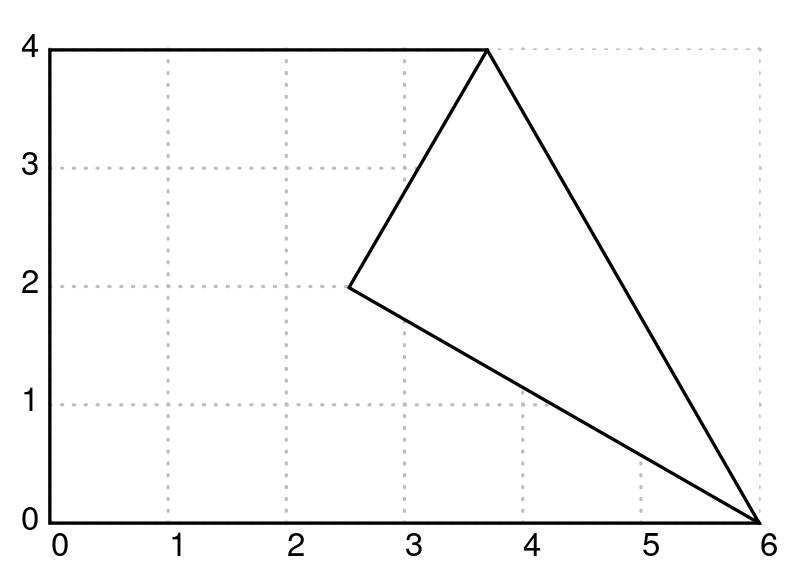
\includegraphics[width=1\textwidth]{306090.png}
            \caption{Resulting Fold}
        \end{figure}

        \begin{figure}[h!]
            \centering
            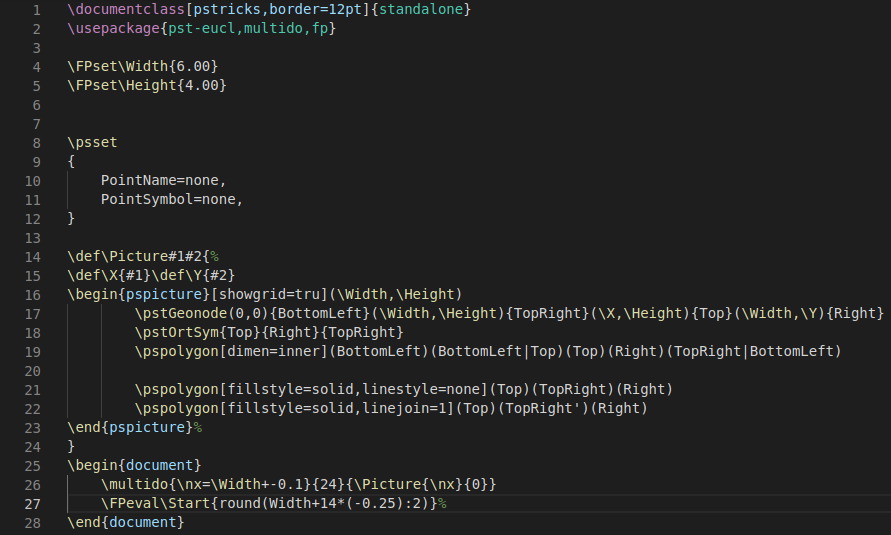
\includegraphics[width=1\textwidth]{origami.png}
            \caption{Code to Generate the Origami Animation}
        \end{figure}

        \newpage
        \begin{proof}
            Consider the diagram below. Notice that the hypotenuse of $\Delta ABC$
            is equal to the height of our paper say $x$ (in this specific case, that is equal to 4).
            It is also clear, that the shorter leg is equal to $\frac{x}{2}$ .
           
            Now, borrowing from plane geometry, it follows that $\Delta ABC$ is a 30-60-90 triangle.

            That fact will imply the following:

            \begin{enumerate}
                \item $\angle CAB = 30^{\circ}$
                \item $\angle DAC = 60^{\circ}$ since $\angle DAB$ is a right triangle
                \item $\angle DAE = \angle EAD = \angle DEA = \angle AEC = 30^{\circ} $ since $\overline{\rm AE}$ is a bisector of 
                $\angle DAC$ and $\angle DEC$
                \item $\angle ADE = 60^{\circ}$ since $\Delta ADE$ is an isoceles triangle.
            \end{enumerate}

            \begin{figure}[h!]
                \centering
                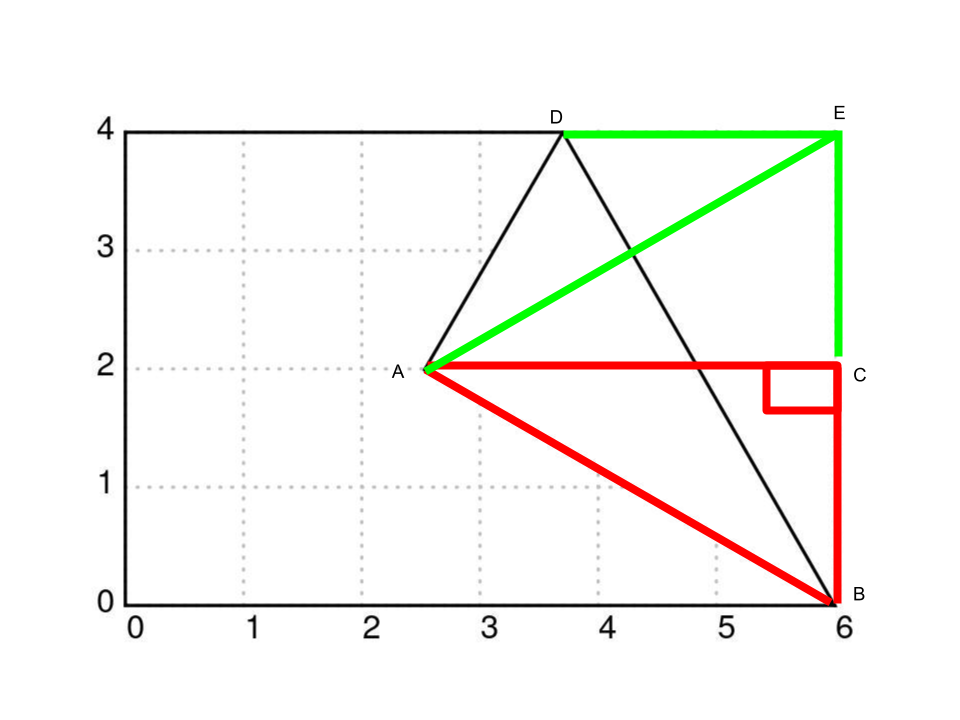
\includegraphics[width=1\textwidth]{306090_1.png}
                \caption{Code to Generate the Origami Animation}
            \end{figure}
            \newpage
            $\therefore \Delta DAB$ is a 30$^{\circ}$ - 60$^{\circ}$ - 90$^{\circ}$ triangle since
            by contruction $\angle DAB$ is a right angle and we have shown that $\angle ADE = 60^{\circ}$ 
            The sum of the angles must be $180^{\circ}$ thereby forcing $\angle DBA = 30^{\circ}$.

        \end{proof}


\end{document}